\section{Скобка Кауфмана и полином Джонса}

\subsection{Скобка Кауфмана}

Это полином, вычисляемый как сумму выражений для разных состояний сглаживания плоской диаграммы узла.
Под сглаживанием понимается замена перекрёстков непересекающимися парами дуг.

\graphicspath{{\currentpath}}

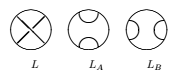
\includegraphics{images/resolve-cross.png}

На картинке показано, как для пересечения L строются сглаживание A и сглаживание B. Их направление определяется относительным положением верхней и нижней линии. Если идти по верхней линии в любую сторону, то область A до перекрёстка будет слева, а после него - справа. Область B, соответственно, наоборот. Выбранный тип сглаживания заменяет перекрёсток на две дуги, проходящие в областях A или B соответственно

Выбирая для каждого перекрёстка способ его разрешения, для диаграммы с n перекрёстками, получаем $2^n$ возможных состояний.
Обозначив для каждого состояния $s$: $\alpha_s$ - число разрешений типа A, $\beta_s$ - число разрешений типа B, $\gamma_s$ - число связных компонент состояния,
запишем:

$$S = \sum_{s} a^{\alpha_s} b^{\beta_s} c^{\gamma_s - 1}$$

- сумма произведений по всем состояниям.

Эта сумма для любых $a$, $b$, $c$ инвариантна относительно второго и третьего движений Рейдемайстера.

Если принять
$$b = a^{-1};\; c = \left(-a^2 - a^{-2}\right);$$
то сумма обратится в сумму Кауфмана или скобку Кауфмана.

$$K = \sum_{s} a^{\alpha_s - \beta_s} \left(-a^2 - a^{-2}\right)^{\gamma_s - 1}.$$

Первое движение Рейдемайтера для суммы Кауфмана эквивалентно умножению на $-a^{\pm 3}$. Где знаки соответствуют знакам крутки получаемого перекрёстка (или противоположны знаку вращение калышки).

\subsection{Число закрученности}

Если выбрать на каждой компоненте зацепления направление обхода, получим ориентированное зацепление. Тогда для каждого перекрёстка можно определить направление крутки - положительное (правое) или отрицательное (левое), сообразно тому, куда крутила бы относительно оси, заданной одной линией, сила приложенная вдоль другой.

Принимая закрученность каждого перекрёстка за $\pm 1$ и просуммировав их, получим число закрученности зацепления $\omega$.

\subsection{Полином Джонса}

Если умножить сумму Кауфмана на $(-a^3)^{-\omega}$, получим многочлен

$$X = (-a^3)^{-\omega}K.$$

Этот многочлен инвариантен относительно всех трёх движений Рейдемайтера.

Если принять
$$a = t^{-\frac{1}{4}};$$
то получим полином Джонса.

Полином Джонса является многочленом Лорана от переменной $t^{\frac{1}{2}}$.